\pdftrailerid{}
\documentclass[10pt,border=1pt]{standalone}
\usepackage[T1]{fontenc}
\usepackage{mathpazo}
\usepackage{amsmath,amssymb}
\usepackage{xcolor}
\usepackage{pgfplots}
\pgfplotsset{compat=1.18}
\usetikzlibrary{shapes.geometric,positioning,arrows.meta,calc}
\definecolor{okorange}{HTML}{E69F00}
\definecolor{oksky}{HTML}{56B4E9}
\definecolor{okgreen}{HTML}{009E73}
\definecolor{okblue}{HTML}{0072B2}
\definecolor{okverm}{HTML}{D55E00}
\definecolor{okpurple}{HTML}{CC79A7}
\colorlet{accent}{okverm}
\pgfplotsset{
  safenest/.style={
    tick label style={font=\footnotesize},
    label style={font=\small},
    title style={font=\small, align=left},
    legend style={font=\footnotesize, draw=none, fill=none, cells={anchor=west}},
    grid style={black!12, line width=0.3pt},
    axis line style={black!70, line width=0.4pt},
    tick style={black!70, line width=0.4pt},
    axis lines*=left,
  },
}
\newlength{\figwidth}
\tikzset{every node/.append style={execute at begin node={\hyphenpenalty=10000\exhyphenpenalty=10000\relax}}}
\setlength{\figwidth}{18.47cm}
\begin{document}
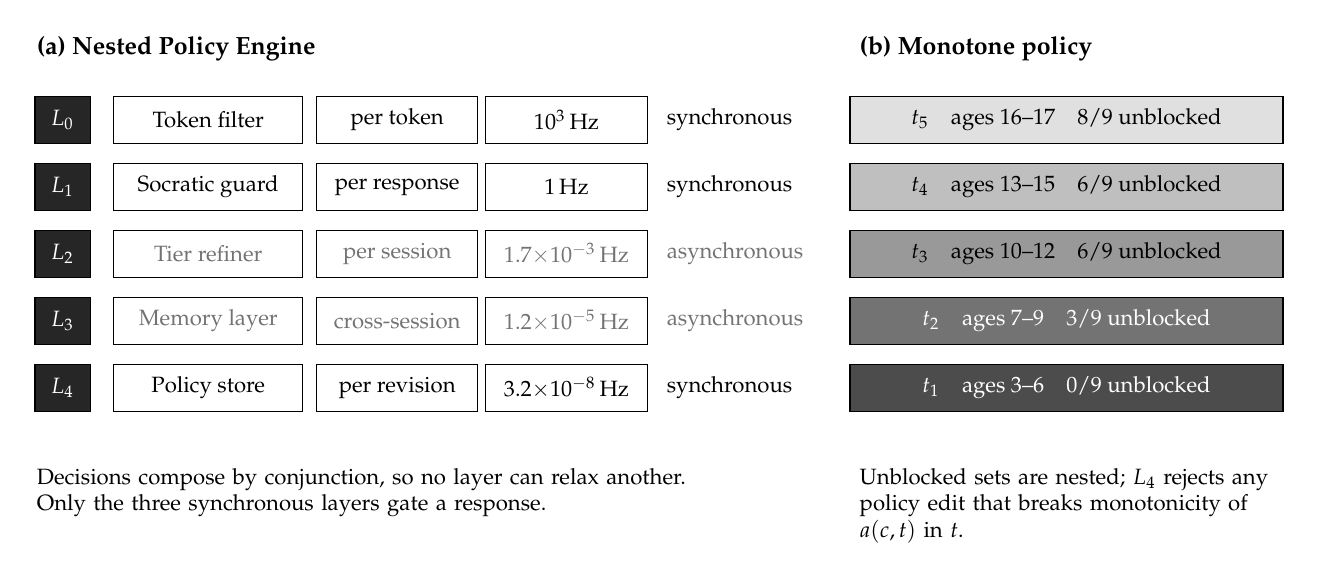
\begin{tikzpicture}[
  lbl/.style={draw, thin, rectangle, minimum width=7mm, minimum height=6mm,
              fill=black!85, text=white, font=\footnotesize},
  lname/.style={draw, thin, rectangle, minimum width=24mm, minimum height=6mm, font=\footnotesize},
  lcell/.style={draw, thin, rectangle, minimum width=20.5mm, minimum height=6mm, font=\footnotesize},
  tierbox/.style={draw, thin, rectangle, minimum width=55mm, minimum height=6mm, font=\footnotesize},
]
\node[font=\small\bfseries, anchor=west] at (-0.45,0) {(a) Nested Policy Engine};
\node[font=\small\bfseries, anchor=west] at (10.0,0) {(b) Monotone policy};
\node[lbl] at (0,-0.90) {$L_0$};
\node[lname] at (1.85,-0.90) {Token filter};
\node[lcell] at (4.25,-0.90) {per token};
\node[lcell] at (6.4,-0.90) {$10^{3}$\,Hz};
\node[font=\footnotesize, anchor=west] at (7.55,-0.90) {synchronous};
\node[lbl] at (0,-1.75) {$L_1$};
\node[lname] at (1.85,-1.75) {Socratic guard};
\node[lcell] at (4.25,-1.75) {per response};
\node[lcell] at (6.4,-1.75) {$1$\,Hz};
\node[font=\footnotesize, anchor=west] at (7.55,-1.75) {synchronous};
\node[lbl] at (0,-2.60) {$L_2$};
\node[lname, text=black!55] at (1.85,-2.60) {Tier refiner};
\node[lcell, text=black!55] at (4.25,-2.60) {per session};
\node[lcell, text=black!55] at (6.4,-2.60) {$1.7{\times}10^{-3}$\,Hz};
\node[font=\footnotesize, text=black!55, anchor=west] at (7.55,-2.60) {asynchronous};
\node[lbl] at (0,-3.45) {$L_3$};
\node[lname, text=black!55] at (1.85,-3.45) {Memory layer};
\node[lcell, text=black!55] at (4.25,-3.45) {cross-session};
\node[lcell, text=black!55] at (6.4,-3.45) {$1.2{\times}10^{-5}$\,Hz};
\node[font=\footnotesize, text=black!55, anchor=west] at (7.55,-3.45) {asynchronous};
\node[lbl] at (0,-4.30) {$L_4$};
\node[lname] at (1.85,-4.30) {Policy store};
\node[lcell] at (4.25,-4.30) {per revision};
\node[lcell] at (6.4,-4.30) {$3.2{\times}10^{-8}$\,Hz};
\node[font=\footnotesize, anchor=west] at (7.55,-4.30) {synchronous};
\node[tierbox, fill=black!12, text=black] at (12.75,-0.90) {$t_5$\quad ages 16--17\quad 8/9 unblocked};
\node[tierbox, fill=black!25, text=black] at (12.75,-1.75) {$t_4$\quad ages 13--15\quad 6/9 unblocked};
\node[tierbox, fill=black!40, text=black] at (12.75,-2.60) {$t_3$\quad ages 10--12\quad 6/9 unblocked};
\node[tierbox, fill=black!55, text=white] at (12.75,-3.45) {$t_2$\quad ages 7--9\quad 3/9 unblocked};
\node[tierbox, fill=black!70, text=white] at (12.75,-4.30) {$t_1$\quad ages 3--6\quad 0/9 unblocked};
\node[font=\footnotesize, anchor=north west, text width=88mm] at (-0.45,-5.2)
  {Decisions compose by conjunction, so no layer can relax another. Only the
   three synchronous layers gate a response.};
\node[font=\footnotesize, anchor=north west, text width=56mm] at (10.0,-5.2)
  {Unblocked sets are nested; $L_4$ rejects any policy edit that breaks
   monotonicity of $a(c,t)$ in $t$.};
\end{tikzpicture}
\end{document}
